
\documentclass[aps,prb,superscriptaddress,twocolumn]{revtex4}
%%%%%%%%%%%%%%%%%%%%%%%%%%%%%%%%%%%%%%%%%%%%%%%%%%%%%%%%%%%%%%%%%%%%%%%%%%%%%%%%%%%%%%%%%%%%%%%%%%%%%%%%%%%%%%%%%%%%%%%%%%%%%%%%%%%%%%%%%%%%%%%%%%%%%%%%%%%%%%%%%%%%%%%%%%%%%%%%%%%%%%%%%%%%%%%%%%%%%%%%%%%%%%%%%%%%%%%%%%%%%%%%%%%%%%%%%%%%%%%%%%%%%%%%%%%%
\usepackage{amsmath}
\usepackage{graphicx}
\usepackage{subfig}

\setcounter{MaxMatrixCols}{10}


\newcommand{\vk}{\ensuremath{\mathbf{k}}}
\providecommand{\vr}{\ensuremath{\mathbf{r}}}
\newcommand{\gk}{\ensuremath{{g}(\mathbf{k})}}
\newcommand{\vp}{\ensuremath{\mathbf{p}}}
\newcommand{\gp}{\ensuremath{{g}(\mathbf{p})}}
\newcommand{\vq}{\ensuremath{\mathbf{q}}}
\newcommand{\Fo}{\ensuremath{\mathbf{F_0}}}
\newcommand{\E}{\ensuremath{\mathbf{E}}}
\newcommand{\A}{\ensuremath{\mathbf{A}}}
\newcommand{\J}{\ensuremath{\mathcal{J}}}
\newcommand{\ket}[1]{\ensuremath{\left|#1\right>}}
\newcommand{\bra}[1]{\ensuremath{\left<#1\right|}}
\newcommand{\twoe}{\ensuremath{2\epsilon_\vk-\E_1}}
\newcommand{\nth}[1]{\ensuremath{\frac{1}{#1}}}
\newcommand{\br}[1]{\ensuremath{\left(#1\right)}}
\newcommand{\mbr}[1]{\ensuremath{\left[#1\right]}}
\newcommand{\bbr}[1]{\ensuremath{\left\{#1\right\}}}
\newcommand{\av}[1]{\ensuremath{\bigl<{#1}\bigr>}}
\newcommand{\avv}[2][\nu]{\av{#1{\lvert{#2}\rvert}#1}}
\newcommand{\avt}[2]{\av{{#1}|{#2}}}
\newcommand{\avtu}[1]{\av{T_\tau#1}}
\newcommand{\zmatrix}{\ensuremath{\br{\begin{smallmatrix}0&0\\0&0\end{smallmatrix}}}}
\newcommand{\fmtrx}[4]{\ensuremath{\br{\begin{smallmatrix}#1&#2\\#3&#4\end{smallmatrix}}}}
\newcommand{\smtrx}[6]{\ensuremath{\br{\begin{smallmatrix}#1&#2\\#3&#4\\#5&#6\end{smallmatrix}}}}
\newcommand{\vz}{\ensuremath{v^{\beta\alpha}_{\vk,\vk}}}
\providecommand{\abs}[1]{\ensuremath{\lvert{#1}\rvert}}
\newcommand{\com}[2]{\ensuremath{\mbr{#1,#2}}}
\newcommand{\D}{\ensuremath{\mathit{D}}}
\providecommand{\hm}{\ensuremath{\frac{\hbar^2}}{2m}}
\providecommand{\pdiff}[2]{\ensuremath{\frac{\partial{#1}}{\partial{#2}}}}
\providecommand{\dpdiff}[2]{\ensuremath{\frac{\partial^2{#1}}{\partial{{#2}^2}}}}
\providecommand{\H}{\ensuremath{\mathcal{H}}}
\providecommand{\wt}[1]{\widetilde{#1}}
\newcommand{\efo}{\epsilon_{F_0}}
\newcommand{\fo}{\ensuremath{\ket{F_0}}}
\renewcommand{\E}{\ensuremath{\mathcal{E}}}


\begin{document}

\title{A Coboson Derivation of Richardson Equations for Cooper pairs}
\author{Monique Combescot}
\affiliation{Department of Physics, University of Illinois at Urbana-Champaign, 1110 W
Green St, Urbana, IL, 61801}
\affiliation{Institut des NanoSciences de Paris, Universite Pierre et Marie Curie, CNRS,
Campus Boucicaut, 140 rue de Lourmel, 75015 Paris}
\author{Guojun Zhu}
\affiliation{Department of Physics, University of Illinois at Urbana-Champaign, 1110 W
Green St, Urbana, IL, 61801}
\author{Walter V. Pogosov}
\affiliation{Institut des NanoSciences de Paris, Universite Pierre et Marie Curie, CNRS,
Campus Boucicaut, 140 rue de Lourmel, 75015 Paris}
\affiliation{Institute for Theoretical and Applied Electrodynamics, Russian Academy of
Sciences, Izhorskaya 13, 125412 Moscow}
\date{\today}

\begin{abstract}
Five years after the milestone paper by Bardeen, Cooper, Schrieffer in which
superconductivity is tackled within the grand canonical ensemble, Richardson
has approached the problem within the canonical ensemble: he succeeded to
write the \textit{exact} form of the Schr\"{o}dinger equation eigenstate for
an arbitrary number of Cooper pairs interacting through the standard BCS
potential. We here rederive his result using the commutation technique we
have recently developed for many-body effects between composite bosons
(cobosons in short). This derivation makes crystal clear that interactions
between Cooper pairs are solely due to the Pauli exclusion principle,
through electron exchanges between pairs. Our procedure also gives hints on
why, as we very recently found, the interaction part of the $N$-pair energy
depends on pair number as $N(N-1)$ only from the dilute to the dense regime
of pairs. In this work, we also briefly discuss the validity of the BCS wave
function ansatz in the light of Richardson exact form.
\end{abstract}

\pacs{}
\maketitle

% Use the \preprint command to place your local institutional report
% number in the upper righthand corner of the title page in preprint mode.
% Multiple \preprint commands are allowed.
% Use the 'preprintnumbers' class option to override journal defaults
% to display numbers if necessary
%\preprint{}

%Title of paper

% repeat the \author .. \affiliation  etc. as needed
% \email, \thanks, \homepage, \altaffiliation all apply to the current
% author. Explanatory text should go in the []'s, actual e-mail
% address or url should go in the {}'s for \email and \homepage.
% Please use the appropriate macro foreach each type of information

% \affiliation command applies to all authors since the last
% \affiliation command. The \affiliation command should follow the
% other information
% \affiliation can be followed by \email, \homepage, \thanks as well.

%\email[]{Your e-mail address}
%\homepage[]{Your web page}
%\thanks{}
%\altaffiliation{}

%Collaboration name if desired (requires use of superscriptaddress
%option in \documentclass). \noaffiliation is required (may also be
%used with the \author command).
%\collaboration can be followed by \email, \homepage, \thanks as well.
%\collaboration{}
%\noaffiliation

% insert suggested PACS numbers in braces on next line

% insert suggested keywords - APS authors don't need to do this
%\keywords{}

%\maketitle must follow title, authors, abstract, \pacs, and \keywords

% body of paper here - Use proper section commands
% References should be done using the \cite, \ref, and \label commands

Although it has been immediately noted that the Pauli exclusion principle
plays a key role in superconductivity, it is quite recently only that the
precise way it transforms a collection of single Cooper pairs into a BCS
condensate, has been really understood. This understanding goes through
handling Cooper pairs not within the grand canonical ensemble as done in the
standard BCS theory, but through the canonical ensemble. The handling of the
Pauli exclusion principle between a fixed number of fermions is however
known to be a formidable problem. Nevertheless, adding fermion pairs one by
one is the unique way to possibly follow the increasing effect of Pauli
blocking when the number of pairs increases.

Five years after the milestone paper on superconductivity by Bardeen,
Cooper, Schrieffer\cite{BCS}, Richardson has derived the form of the exact
eigenstate of the Schr\"{o}dinger equation for a fixed number of Cooper pairs%
\cite{Richardson1,Richardson2}. In the case of $N$ pairs, it reads in terms
of $N$ parameters, $R_{1}$,... $R_{N}$ which are solutions of $N$ coupled
non-linear equations, the energy of these $N$ pairs reading as $\mathbf{E}%
_{N}=R_{1}+...+R_{N}$. Although this result is definitely quite smart, to
use it in practice, is not that easy: Indeed, these equations have no
compact analytical solution, so that they are commonly approached
numerically only. This is probably why they have not had so far the
attention they deserve among the superconductor community. Nowadays, they
are commonly used to numerically study properties of small superconducting
particles with an accountable number of electron pairs.

Last year, we analyzed a connection between the two classical problems: the
one-pair problem solved by Cooper and the many-pair BCS configuration. In
both cases, there is a "frozen" core of noninteracting electrons. There is
also a potential layer above this core, where an attraction between up and
down spin electrons is localized. In one-pair problem this layer contains
only one correlated electron pair, while in the standard BCS theory the
layer is half-filled (usually this is interpreted in terms of the extension
of the potential layer symmetrically over both sides of the Fermi level,
such an understanding being of course fully equivalent with our approach).
By adding more and more pairs into this layer, one can continuosly reach BCS
regime starting from the one-pair limit. Although manipulation of this kind
can hardly been performed experimentally (at least, nowadays), it allows one
to see the evolution of energetical spectrum with changing the filling of
the potential layer and thus to deeper understand the role of the Pauli
exclusion principle for Cooper pairs. In addition, this procedure can be
considered as a simple and well-defined toy model for the BEC-BCS crossover
problem, since by changing the number of pairs in the potential layer one
can tune their overlap (This procedure has to be contrasted with the one of
Ref. [Leggett], where the overlap was changed by tuning the interaction
between pairs). The crossover thus occurs only for those pairs which are
inside the potential layer. Notice that the BEC-BCS crossover problem has
not \ been solved yet \textit{in a fully controllable way} even for the
"reduced" BCS interaction between up and down spin electrons, which couples
only fermions with opposite spins and momenta. In contrast with variational
BCS-like theories [Eagles, Leggett], Richardson's approach provides an exact
solution to the many-pair Schr\"{o}dinger equation and thus makes it
possible to tackle the most interesting domain of the phase diagram, which
is in the middle between the dilute and dense regimes of pairs. The interest
to his domain is due to the fact that, as it was realized long time ago, the
BCS ansatz for the wave function can collapse in this region [Leggett].
Notice that the crossover problem within Richardson equations was studied in
Ref. [Dukelsky] by using an assumption that ground-state $R$'s form a single
arc in the complex plane and by using a continous approximation.

Although Richardson procedure drastically simplifies quantum many-body
problem, the resolution of Richardson equations is a quite complicated
problem. By turning to the dimensionless form of of these equations we have
found an analytical way to solve these equations in the dilute regime of
pairs. We then see that these equations do have a small parameter: It is $1/{%
N_{c}}$ where $N_{c}$ is the number of Cooper pairs for which overlap
between pairs starts. This allowed us to demonstrate in the dilute limit on
the single Cooper pair scale, i.e., for $N/N_{c}$ small, that the energy of $%
N$ Cooper pairs reads as 
\begin{equation}
\mathcal{E}_{N}=N\left[ \left( 2\epsilon _{F_{0}}+\frac{N-1}{\rho _{0}}%
\right) )-\epsilon _{c}\left( 1-\frac{N-1}{N_{\Omega }}\right) \right]
\label{eq:eN}
\end{equation}%
$\epsilon _{F_{0}}$ is the Fermi level of the Fermi sea $\left\vert
F_{0}\right\rangle $ which does not feel the attractive potential, $\rho
_{0} $ is the density of states, taken as constant within the potential
layer. $N_{\Omega }=\rho _{0}\Omega $ is the number of pair states in this
layer, $\Omega $ being the potential layer extension. $\epsilon _{c}\approx
2\Omega \exp \left( -2/\rho _{0}V\right) $ is the single pair binding
energy, the potential amplitude being V.

Although our actual derivation imposes $N/N_{c}$ small, it is quite
remarkable to note that this result is also valid in the dense BCS regime,
where pairs strongly overlap. Indeed the first term of Eq.\eqref{eq:eN} is
the exact energy of $N$ pairs in a normal state, since it is nothing but 
\begin{equation}
2\epsilon _{F_{0}}+\left( 2\epsilon _{F_{0}}+1/\rho _{0}\right) +\cdots
\;+\left( 2\epsilon _{F_{0}}+(N-1)/\rho _{0}\right) =\mathcal{E}_{N}^{\text{(%
}normal)}
\end{equation}%
For a number of pairs corresponding to fill half the potential layer, which
is the precise BCS configuration, Eq.\eqref{eq:eN} gives a condensation
energy equal to 
\begin{equation}
\mathcal{E}_{N}-\mathcal{E}_{N}^{\text{(}normal)}=\frac{N_{\Omega }}{2}\frac{%
\epsilon _{c}}{2}=\frac{1}{2}\rho _{0}\Omega ^{2}e^{-2/\rho _{0}V}
\end{equation}%
This result exactly matches the one derived within the grand canonical
ensemble, namely $\rho _{0}\Delta ^{2}/2$ where the gap $\Delta $ reads as $%
2\omega _{c}\exp \left( -1/\rho _{0}V\right) $ since $2\omega _{c}$ is the
potential layer extension $\Omega $. By considering BCS configuration with
arbitrary, but large $N$ ($N\gg \Delta $), we have also shown that Eq.%
\eqref{eq:eN} remains valid here as well.

The canonical approach we have used to reach Eq.\eqref{eq:eN}, based on the
Richardson equations, has the great advantage to trace the evolution of the
ground state energy with adding pairs one by one. We then see that it is
reasonable to associate the last term in the righ-hand side of Eq.%
\eqref{eq:eN}, i.e., $\epsilon _{c}\left[ 1-\left( N-1\right) /N_{\Omega }%
\right] $, with the "pair binding energy" in the $N$-pair configuration
(dressed by the Fermi sea). Indeed, at $N=1$ this quantity matches with the
single-pair binding energy as found by Cooper, while in the dense regime it
gives the condensation energy per pair. Therefore, by using this quantity
one can understand dilute and dense regimes of pairs on the same footing.

It is straightforward to realize that the pair binding energy, as defined
above, decreases when $N$ increases. This decrease is caused entirely by
Pauli blocking that decreases the number of available one-electron states in
the potential layer with the growth of $N$. A very pictural way to
understand the binding energy decreases when $N$ increases is through the
so-called "moth-eaten" effect: when pairs are added to $\left\vert
F_{0}\right\rangle $, they are "eating" one by one, like little moths, the
states in the potential layer which are available to form a bound state. As
a result of this available state decrease, the bound state energy can only
decrease. Our understanding of the pair binding energy is in a contrast with
the common belief that in the dense BCS configuration, the Cooper pair
binding energy is of the order of the gap $\Delta $, which is far larger
than $\epsilon _{c}$. This interpretation is obtained by splitting the
condensate energy $\rho _{0}\Delta ^{2}/2$ as $(\rho _{0}\Delta )\Delta $
within an "irrelevant" $1/2$ prefactor. This deliberatly assigns a pair
energy equal to the gap, the number of pairs to fit the condensation energy
then being the number of pair $\rho _{0}\Delta $ in a gap layer. These $\rho
_{0}\Delta $ pairs actually are "virtual pairs", as named by Schrieffer.
Their number is far smaller than the number of pairs $N_{\Omega }/2$ feeling
the potential. This obviously makes their energy far larger than the energy $%
\epsilon _{c}/2$ of the real pairs. These virtual pairs in fact correspond
to excitations accross the Fermi sea $\left\vert F\right\rangle $ made of $%
N+N_{0}$ \textit{noninteracting} pairs, $N_{0}$ being the number of pairs in
the frozen sea $\left\vert F_{0}\right\rangle $. The concept of vurtual
pairs has physical meaning in the dense regime of pairs only, since in the
dilute regime the Fermi level of noninteracting electrons is completely
washed out, so that all the pairs are essentially excited above this level.
Thus this concept somehow masks a link with the dilute regime of pairs. This
was probably one of the reasons for the Schrieffer's statement that the
isolated pair concept has a little meaning in the dense regime of pairs
[Schrieffer]. This point of view was however questened by Leggett who has
argued that pairs in the dense limit in many aspects are similar to giant
molecules [Leggett]. Notice that, in general, the problem of physical
interpretation of the paired state nature has a long prehistory.

Since the key role of Pauli blocking in superconductivity is enlightened by
our expression of the $N$-pair energy Eq.\eqref{eq:eN} obtained by solving
Richardson equations, it can be of interest to precisely see the parts in
these equations which directly come from the Pauli exclusion principle.

In our recent works on the many-body physics of composite bosons, we have
proposed a "commutation technique" which allows us to evidence the effects
of Pauli blocking between the fermionic components of these composite
bosons. They appear through "Pauli scatterings" which describe fermion
exchanges in the absence of fermion interaction. These dimensionless Pauli
scatterings, mixed with energy-like scatterings associated to interactions
between fermionic components, allow us to deal with fermion exchanges
between composite bosons (cobosons in short) in an exact way. For review on
this formalism and its applications to the many-body physics of
semiconductor excitons, see ref \cite%
{CobosonPhysicsReports,CobosonCalculation}.

In this paper, we first develop such a commutation technique for up and down
electron pairs with zero total momentum. We then use it to derive in a quite
compact way, the form of the exact eigenstate for $N$ pairs interacting
through the reduced BCS potential. The Richardson equations readily follow
from this approach. Its main advantage is to possibly trace back in a
transparent way, the terms in these equations which directly come from the
Pauli exclusion principle: they are those in $R_i-R_j$. They actually come
from the non-zero values of Pauli scatterings for fermion exchanges between
cobosons made of free electron pairs.

The paper is organized as following:

In section \ref{sec:beta}, we derive the commutation technique for free
electron pairs and its associated Pauli and interaction scatterings.

In section \ref{sec:rich}, we use this technique to get the form of the
exact eigenstate for $N=2,3,\cdots$ pairs interacting through the reduced
BCS potential, in order to see how the solution for general $N$ develops. We
then analyze the increasing role Pauli blocking in these solutions.

In section \ref{sec:conn}, we discuss possible connection between this exact
solution and the BCS ansatz for condensed pairs

\section{Commutation Technique for free fermion pairs\label{sec:beta}}

\subsection{Exchange between free fermion pairs}

We consider cobosons made of free fermion pairs having a zero total
momentum. 
\begin{equation}
\beta^{\dagger}_\vk=a^{\dagger}_{\mathbf{k} }b^{\dagger}_{-\mathbf{k} }
\end{equation}
These pairs only have one degree of freedom, namely $k$, by contrast to the
most general fermion pairs $a^{\dagger}_{\mathbf{k} _1}b^{\dagger}_{\mathbf{k%
} _2}$ which have two. In the case of Cooper pairs, these fermions are up
and down spin electrons. The fermion operators ($a^{\dagger}_{\mathbf{k}
^{\prime}}$,$a^{\dagger}_{\mathbf{k} }$) and ($b^{\dagger}_{\mathbf{k}
^{\prime}}$,$b^{\dagger}_{\mathbf{k} }$) anticommute while $a^{\dagger}_{%
\mathbf{k} ^{\prime}}$ and $b^{\dagger}_{\mathbf{k} }$ commute or
anticommute depending if the two fermions have the same or a different
nature. However, as easy to check, this does not affect the commutation
relations between fermion pair operators. For two creation operators, these
are 
\begin{equation}  \label{eq:bCom}
\left[\beta^{\dagger}_{\mathbf{k} ^{\prime}},\beta^{\dagger}_{\mathbf{k} }%
\right]  =0
\end{equation}
It is worth noting that while $\left(a^{\dagger}_{\mathbf{k} }\right) ^2=0$
simply follows from the anticommutation of the $a^{\dagger}_{\mathbf{k} }$
operators, the cancellation of $\left(\beta^{\dagger}_{\mathbf{k} }\right) ^2
$ does not follow from Eq.\eqref{eq:bCom}, but from the fact that $%
\left(\beta^{\dagger}_{\mathbf{k} }\right) ^2$ contains $\left(a^{\dagger}_{%
\mathbf{k} {}}\right) ^2$. The cancellation of $\left(\beta^{\dagger}_{%
\mathbf{k} }\right) ^2$ which comes from Pauli blocking, seems to be lost
when turning from single fermion operators to pair operators. We will
however see that this blocking is yet preserve in the commutaion algebra of
free fermion pairs we are developping.

For creation and annihilation operators, $\left[a^{}_{\mathbf{k}
^{\prime}},a^{\dagger}_{\mathbf{k} {}}\right]  =\delta_{\mathbf{k} ^{\prime}%
\mathbf{k} }$ leads to 
\begin{equation}  \label{eq:betacom}
\left[\beta_{\mathbf{k} ^{\prime}},\beta^{\dagger}_{\mathbf{k} }\right] 
=\delta_{\mathbf{k} ^{\prime}\mathbf{k} }-\mathit{D} _{\mathbf{k} ^{\prime}%
\mathbf{k} }
\end{equation}
the deviation-from-boson operator $\mathit{D} _{\mathbf{k} ^{\prime}\mathbf{k%
} }$ being defined as 
\begin{equation}  \label{eq:D}
\mathit{D} _{\mathbf{k} ^{\prime}\mathbf{k} }=\delta_{\mathbf{k} ^{\prime}%
\mathbf{k} }\left(a^{\dagger}_{\mathbf{k} \uparrow}a^{}_{\mathbf{k}
\uparrow}+a^{\dagger}_{-\mathbf{k} \downarrow}a^{}_{-\mathbf{k}
\downarrow}\right) 
\end{equation}
This operator which would reduce to zero if the fermion pairs were
elementary bosons, allows us to generate the Pauli scatterings for fermion
exchanges. They are formally defined through 
\begin{equation}
\left[\mathit{D} _{\mathbf{k} ^{\prime}_1\mathbf{k} _1},\beta^{\dagger}_{%
\mathbf{k} _2}\right]  =\sum_{\mathbf{k} ^{\prime}_2}\left\{\lambda\left(%
\begin{smallmatrix}\vk'_2&\vk_2\\\vk'_1&\vk_1\end{smallmatrix}\right) 
+\left(\mathbf{k} ^{\prime}_1\leftrightarrow\mathbf{k} ^{\prime}_2\right)
\right\} \beta^{\dagger}_{\mathbf{k} ^{\prime}_2}
\end{equation}
By noting that

\begin{equation}  \label{eq:aBeta}
\left[a^{\dagger}_{\mathbf{k} }a^{}_{\mathbf{k} },\beta^{\dagger}_{\mathbf{p}
}\right]  =\delta_{\mathbf{k} \mathbf{p} }\beta^{\dagger}_{\mathbf{p} }=%
\left[b^{\dagger}_{-\mathbf{k} }b^{}_{-\mathbf{k} },\beta^{\dagger}_{\mathbf{%
p} }\right]  
\end{equation}
it is easy to show that 
\begin{equation}  \label{eq:Dcom}
\left[\mathit{D} _{\mathbf{k} ^{\prime}_1\mathbf{k} _1},\beta^{\dagger}_{%
\mathbf{k} _2}\right]  =2\beta^{\dagger}_{\mathbf{k} _2}\delta_{\mathbf{k} _1%
\mathbf{k} _2}\delta_{\mathbf{k} ^{\prime}_1,\mathbf{k} _2}
\end{equation}
So that we are led to identify the Pauli scattering with the following
product of Kronecker symbols 
\begin{equation}  \label{eq:pauliscattering}
\lambda\left(\begin{smallmatrix}\vk'_2&\vk_2\\\vk'_1&\vk_1\end{smallmatrix}%
\right)  =\delta_{\mathbf{k} ^{\prime}_1\mathbf{k} _1}\delta_{\mathbf{k}
^{\prime}_2\mathbf{k} _2}\delta_{\mathbf{k} _1\mathbf{k} _2}
\end{equation}
Actually, this is just the value we expect for the scattering associated to
fermion exchanges between $\left(\mathbf{k} _1,\mathbf{k} _2\right) $ pairs,
as visualized by the diagram of fig (\ref{fig:lambda}). Indeed from this
diagram, it is clear that we must have $\left(\mathbf{k} ^{\prime}_1=\mathbf{%
k} _1,\mathbf{k} ^{\prime}_2=\mathbf{k} _2\right) $ and $\left(-\mathbf{k}
^{\prime}_2=-\mathbf{k} _1,-\mathbf{k} ^{\prime}_1=-\mathbf{k} _2\right) $:
this just gives $\delta_{\mathbf{k} ^{\prime}_1\mathbf{k} _1}\delta_{\mathbf{%
k} ^{\prime}_2\mathbf{k} _2}\delta_{\mathbf{k} _1\mathbf{k} _2}$ in
agreement with Eq.\eqref{eq:pauliscattering}.

\begin{figure}[htb]
\caption{Shiva diagram of free pairs }\centering
\par
 % \subfloat[][]{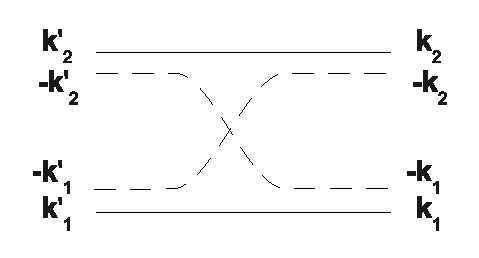
\includegraphics[width=0.3\textwidth]{lambda1.eps}\label{fig:lambda}}\qquad
% \subfloat[][]{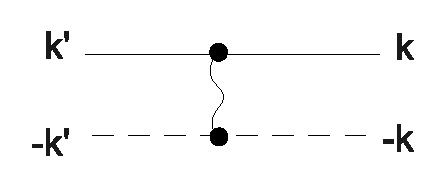
\includegraphics[width=0.3\textwidth]{direct1.eps}\label{fig:direct}}\\
 % \subfloat[][]{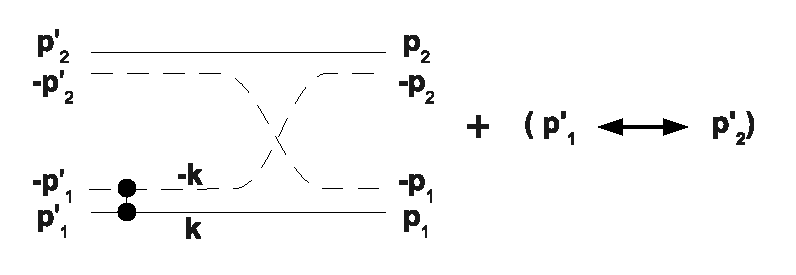
\includegraphics[width=0.4\textwidth]{chi1.eps}\label{fig:chi}} 
\par
\begin{description}
\item[\subref{fig:lambda}] Pauli scattering $\lambda\left(%
\begin{smallmatrix}\vk'_2&\vk_2\\\vk'_1&\vk_1\end{smallmatrix}\right)  $ for
electron exchange between two free pairs $\left(\mathbf{k} _1,\mathbf{k}
_2\right) $, as given by Eq.\eqref{eq:pauliscattering}. Up spin electrons
are represented by solid lines, down spin electrons by dashed lines. 
\par
\item[\subref{fig:direct}] The BCS potential given in Eq.\eqref{eq:vbcs}
transforms a $\mathbf{k} $ pair into a $\mathbf{k} ^{\prime}$ pair, with a
constant scattering $-V$, in the case of a separable potential $v_{\mathbf{k}
^{\prime}\mathbf{k} }=-V\,w_{\mathbf{k} ^{\prime}}w_{\mathbf{k} }$.
\par
\item[\subref{fig:chi}] Interaction scattering $\chi\left(%
\begin{smallmatrix}\vp'_2&\vp_2\\\vp'_1&\vp_1\end{smallmatrix}\right)  $
between two free pairs, as given in Eq.\eqref{eq:interactSc}. Since the BCS
potential acts within one pair only, the interaction between two pairs can
only come from exchange induced by the Pauli exclusion principle. 
\end{description}

\end{figure}

\subsection{Interaction between free fermion pairs}

To get the interaction scatterings associated to fermion interaction, we
first note that for a free fermion hamiltonian 
\begin{equation}  \label{eq:h0}
H_0=\sum{\epsilon_\vk\left(a^{\dagger}_{\mathbf{k} } a^{}_{\mathbf{k}
}+b^{\dagger}_{\mathbf{k} } b^{}_{\mathbf{k} }\right) }
\end{equation}
Eq.\eqref{eq:aBeta} readily gives 
\begin{equation}  \label{eq:betaH}
\left[H_0,\beta^{\dagger}_\vp\right]  =2\epsilon_\vp\beta^{\dagger}_\vp
\end{equation}

In the case of present interest, these fermion pairs interact through the
standard BCS-like (1x1) potential in which the fermion $\mathbf{k} $ only
interacts with the fermion $\left(-\mathbf{k} \right) $ of the other
species. This potential reads 
\begin{equation}  \label{eq:vbcs}
V_{BCS}=\sum{v_{\mathbf{k} ^{\prime}\mathbf{k} }\beta^{\dagger}_{\mathbf{k}
^{\prime}}\beta^{}_{\mathbf{k} }}
\end{equation}
It is represented by the diagram of Fig. \ref{fig:direct}. For this (1x1)
potential, we do have 
\begin{equation}  \label{eq:vbeta}
\left[V_{BCS},\beta^{\dagger}_\vp\right] 
=\gamma^{\dagger}_\vp+V^{\dagger}_\vp
\end{equation}
in which we have $\gamma^{\dagger}_\vp=\sum_\vk\beta^{\dagger}_\vk{}v_{%
\mathbf{k} \mathbf{p} }$. The "creation potential" for the free fermion pair 
$\mathbf{p} $ appears to be 
\begin{equation}  \label{eq:betaV}
V^{\dagger}_\vp=-{\gamma^{\dagger}_\vp}\left(a^{\dagger}_{\mathbf{p} }a^{}_{%
\mathbf{p} }+b^{\dagger}_{-\mathbf{p} }b^{}_{-\mathbf{p} }\right) 
\end{equation}

While the $\gamma^{\dagger}_\vp$ part of Eq.\eqref{eq:vbcs} commutes with $%
\beta^{\dagger}_\vp$, this is not so for the creation potential $%
V^{\dagger}_\vp$. Its commutator precisely reads 
\begin{equation}  \label{eq:vpotbeta}
\left[V^{\dagger}_{\mathbf{p} _1},\beta^{\dagger}_{\mathbf{p} _2}\right] 
=-2\delta_{\mathbf{p} _1\mathbf{p} _2}\gamma^{\dagger}_{\mathbf{p}
_1}\beta^{\dagger}_{\mathbf{p} _1}
\end{equation}
This allows us to identify the interaction scattering for free pairs,
formally defined as 
\begin{equation}  \label{eq:vBeta}
\left[V^{\dagger}_{\mathbf{p} _1},\beta^{\dagger}_{\mathbf{p} _2}\right] 
=\sum\chi\left(\begin{smallmatrix}\vp'_2&\vp_2\\\vp'_1&\vp_1\end{smallmatrix}%
\right)  \beta^{\dagger}_{\mathbf{p} ^{\prime}_1}\beta^{\dagger}_{\mathbf{p}
^{\prime}_2}
\end{equation}
with a sequence of one (2x2) fermion pair exchange and one (1x1) fermion
pair interaction. Indeed 
\begin{equation}  \label{eq:interactSc}
\begin{split}
\chi\left(\begin{smallmatrix}\vp'_2&\vp_2\\\vp'_1&\vp_1\end{smallmatrix}%
\right)  &=-\sum_\vk\left\{v_{\mathbf{p} ^{\prime}_1\mathbf{k} }\lambda\left(%
\begin{smallmatrix}\vp'_2&\vp_2\\\vk&\vp_1\end{smallmatrix}\right)  +\left(%
\mathbf{p} ^{\prime}_1\leftrightarrow\mathbf{p} ^{\prime}_2\right) \right\} 
\\
&=-\left(v_{\mathbf{p} ^{\prime}_1,\mathbf{p} _1}\delta_{\mathbf{p}
^{\prime}_2,\mathbf{p} _2}+v_{\mathbf{p} ^{\prime}_2,\mathbf{p} _2}\delta_{%
\mathbf{p} ^{\prime}_1,\mathbf{p} _1}\right) \delta_{\mathbf{p} _2,\mathbf{p}
_1}
\end{split}%
\end{equation}
This interaction scattering is visualized by the diagram of Fig \ref{fig:chi}%
: the free pairs $\mathbf{p} ^{\prime}_1$ and $\mathbf{p} ^{\prime}_2$ first
exchange a fermion. As for any exchange, this brings a minus sign. In a
second step, the fermions of one of the two pairs interact via the BCS
potential. It is of importance to note that since the potential has a (1x1)
structure, the (2x2) interaction between two pairs can only result from
fermion exchange between pairs, i.e., Pauli blocking.

We are now going to use this commutation formalism to derive the Richardson
equations for Cooper pairs.

\section{Richardson equations for Cooper pairs\label{sec:rich}}

In order to better grasp how these equations develop, let us consider an
increasing number of pairs.

\subsection{One pair}

We consider a state in which one free pair $\mathbf{k} _1$ is added to a
frozen Fermi sea $\left|F_0\right> $ which does not feel the BCS potential.
This means that the $v_{\mathbf{k} ^{\prime}\mathbf{k} }$ prefactors in Eq.%
\eqref{eq:vbcs} cancel for all $\mathbf{k} $ belonging to $\left|F_0\right> $%
. Note that such a "one-pair" state actually contains $N_0+1$ fermion pairs, 
$N_0$ being the number of pairs in the frozen sea. So that this state is in
fact a many-body state, but in the most simple sense since the Fermi sea $%
\left|F_0\right> $ is just there to block states by the Pauli exclusion
principle. This Fermi sea also brings a finite density of state for all the
states above it. This is actually crucial in order to have a bound state,
even for an extremely small attracting BCS potential as evidenced below.

Due to Eqs.(\ref{eq:betaH},\ref{eq:vbeta}), the hamiltonian $H=H_0+V_{BCS}$
acting on this one free pair state gives, by taking the zero energy such
that $H\left|F_0\right> =H_0\left|F_0\right> =0$ 
\begin{equation}
H\beta^{\dagger}_\vk\left|F_0\right>  =\left[H,\beta^{\dagger}_\vk\right] 
\left|F_0\right> 
=\left(2\epsilon_\vk\beta^{\dagger}_\vk+\gamma^{\dagger}_\vk+V^{\dagger}_\vk%
\right) \left|F_0\right>  
\end{equation}
We then note that, due to the $v_{\mathbf{k} \mathbf{p} }$ factor included
in the $\gamma^{\dagger}_{\mathbf{k} }$ part of $V^{\dagger}_\vk$ (see Eq.(%
\ref{eq:betaV})), the creation potential $V^{\dagger}_\vk$ acting on $%
\left|F_0\right> ${\ }gives zero.

If we now substract $\mathbf{E} _1\beta^{\dagger}_\vk\left|F_0\right>  $ to
the two sides of the above equation and divide the resulting equation by $%
\left(2\epsilon_\vk-\mathbf{E} _1\right) $, we find 
\begin{equation}  \label{eq:HE1}
) (H-\mathbf{E} _1)\frac{1}{2\epsilon_\vk-\mathbf{E} _1} \beta^{\dagger}_\vk%
\left|F_0\right>  =\beta^{\dagger}_\vk\left|F_0\right>  +\frac{1}{%
2\epsilon_\vk-\mathbf{E} _1} \gamma^{\dagger}_\vk\left|F_0\right>  
\end{equation}

To go further and possibly get the one-pair eigenstate of the hamiltonian $H$
in an analytical form, it is necessary to approximate the BCS potential
coupling by $v_{\mathbf{k} \mathbf{p} }=-V\,w_\vk{}w_\vp$, the $w_\vk$'s
being moreover such that $w_\vk^2=w_\vk$. This yields 
\begin{equation}  \label{eq:gammaBeta}
\gamma^{\dagger}_\vk=-V\,w_\vk\beta^{\dagger}\quad\quad\beta^{\dagger}=\sum_%
\vp{}w_\vp\beta^{\dagger}_\vp
\end{equation}
If we then multiply Eq.\eqref{eq:HE1} by $w_\vk$ and sum over $\mathbf{k} $,
we find 
\begin{equation}
(H-\mathbf{E} _1)B^{\dagger}(\mathbf{E} _1)\left|F_0\right>  =\left(1-V\sum{%
\frac{w_\vk}{2\epsilon_\vk-\mathbf{E} _1}}\right)
\beta^{\dagger}\left|F_0\right>  
\end{equation}
in which we have set 
\begin{equation}  \label{eq:B}
B_\vk^{\dagger}(E)=\frac{w_\vk}{2\epsilon_\vk-E}\beta^{\dagger}\quad\quad
B^{\dagger}(E)=\sum_\vk{B_\vk^{\dagger}(E)}
\end{equation}
Eq.(23) readily shows that the linear combination $B^{\dagger}(\mathbf{E} _1)
$ of one-pair operators generates the one-pair eigenstate $B^{\dagger}(%
\mathbf{E} _1)\left|F_0\right>  $ of the hamiltonian $H$ with the energy $%
\mathbf{E} _1$, provided that this energy is such that 
\begin{equation}  \label{eq:SchOne}
1=V\sum_\vk{\frac{w_\vk}{2\epsilon_\vk-\mathbf{E} _1}}
\end{equation}
This is nothing but the well-known equation for the single pair energy
derived by Cooper.

\subsection{Two pairs}

Let us now consider two pairs. Eqs.(\ref{eq:betaH},\ref{eq:vbeta}) yield 
\begin{equation}  \label{eq:SchTwo}
\begin{split}
H\beta^{\dagger}_{\mathbf{k} _1}\beta^{\dagger}_{\mathbf{k}
_2}\left|F_0\right>   &=\left(\left[H,\beta^{\dagger}_{\mathbf{k} _1}\right]
\beta^{\dagger}_{\mathbf{k} _2}+\beta^{\dagger}_{\mathbf{k} _1}\left[%
H,\beta^{\dagger}_{\mathbf{k} _2}\right]  \right) \left|F_0\right>   \\
&=\left(2\epsilon_{\mathbf{k} _1}+2\epsilon_{\mathbf{k} _2}\right)
\beta^{\dagger}_{\mathbf{k} _1}\beta^{\dagger}_{\mathbf{k}
_2}\left|F_0\right>  +\left|v_{\mathbf{k} _1\mathbf{k} _2}\right> 
\end{split}%
\end{equation}
where $\left|v_{\mathbf{k} _1\mathbf{k} _2}\right> $ comes from interactions
among the $\left(\mathbf{k} _1,\mathbf{k} _2\right) $ pairs induced by the
BCS potential. Its precise value is 
\begin{equation}
\left|v_{\mathbf{k} _1\mathbf{k} _2}\right> =\left(\gamma^{\dagger}_{\mathbf{%
k} _1}\beta^{\dagger}_{\mathbf{k} _2}+\gamma^{\dagger}_{\mathbf{k}
_2}\beta^{\dagger}_{\mathbf{k} _1}+V^{\dagger}_{\mathbf{k}
_1}\beta^{\dagger}_{\mathbf{k} _2}\right) \left|F_0\right>  
\end{equation}
Eq. \eqref{eq:interactSc} allows us to write the last term of $\left|v_{%
\mathbf{k} _1\mathbf{k} _2}\right> $ as 
\begin{equation}
V^{\dagger}_{\mathbf{k} _1}\beta^{\dagger}_{\mathbf{k} _2}\left|F_0\right>  =%
\left[V^{\dagger}_{\mathbf{k} _1},\beta^{\dagger}_{\mathbf{k} _2}\right] 
\left|F_0\right>  = \sum_{\mathbf{p} ^{\prime}_1\mathbf{p}
^{\prime}_2}\chi\left(\begin{smallmatrix}\vp'_2&\vk_2\\\vp'_1&\vk_1%
\end{smallmatrix}\right)  \beta^{\dagger}_{\mathbf{p} ^{\prime}_1}\beta^{%
\dagger}_{\mathbf{p} ^{\prime}_2}\left|F_0\right>  
\end{equation}
So that $\left|v_{\mathbf{k} _1\mathbf{k} _2}\right> $ can be visualized by
the diagram of Fig. \ref{fig:twoP}. This diagram evidences the fact that,
due to the (1x1) form of the BCS potential, the two pairs $\mathbf{k} _1$
and $\mathbf{k} _2$ interact by fermion exchange only, as a result of the
Pauli exclusion principle.

\begin{figure}[htb]
%   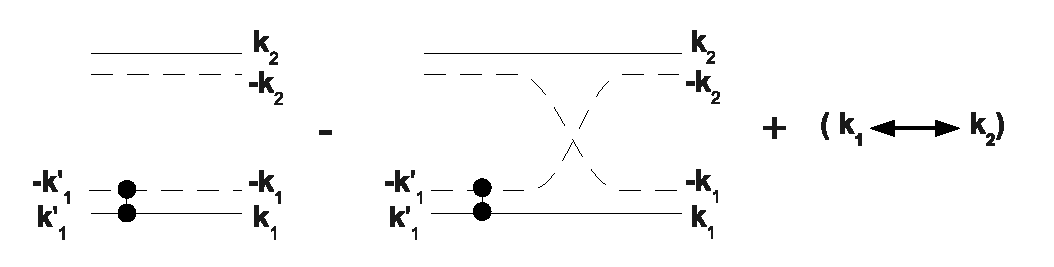
\includegraphics[width=0.4\textwidth]{twoPair.eps}
\caption{Shiva diagram of two pairs }
\label{fig:twoP}
\end{figure}

By using the value of the interaction scattering given in Eq.%
\eqref{eq:vpotbeta}, we find that $\left|v_{\mathbf{k} _1\mathbf{k}
_2}\right> $ is given by 
\begin{equation}
\left|v_{\mathbf{k} _1\mathbf{k} _2}\right> =-V\left(w_{\mathbf{k}
_1}\beta^{\dagger}_{\mathbf{k} _2}+w_{\mathbf{k} _2}\beta^{\dagger}_{\mathbf{%
k} _1}-2\delta_{\mathbf{k} _1\mathbf{k} _2}w_{\mathbf{k} _1}\beta^{\dagger}_{%
\mathbf{k} _1}\right) \beta^{\dagger}\left|F_0\right>  
\end{equation}

To go further, we substract $\mathbf{E} _2\beta^{\dagger}_{\mathbf{k}
_1}\beta^{\dagger}_{\mathbf{k} _2}\left|F_0\right>  $ to the two sides of Eq.%
\eqref{eq:SchTwo}, with $\mathbf{E} _2$ written as $R_1+R_2$ and we multiply
the resulting equation by $w_{\mathbf{k} _1}w_{\mathbf{k} _2}/\left(2%
\epsilon_{\mathbf{k} _1}-R_1\right) \left(2\epsilon_{\mathbf{k}
_2}-R_2\right) $. This gives

\begin{multline}  \label{eq:SchTwo2}
(H-\mathbf{E} _2)B^{\dagger}_{\mathbf{k} _1}(R_1)B^{\dagger}_{\mathbf{k}
_2}(R_2)\left|F_0\right>   = \\
\left\{B^{\dagger}_{\mathbf{k} _1}(R_1)\left(w_{\mathbf{k}
_2}\beta^{\dagger}_{\mathbf{k} _2}-\frac{Vw_{\mathbf{k} _2}}{2\epsilon_{%
\mathbf{k} _2}-R_2}\beta^{\dagger}\right)  +(1\leftrightarrow2)\right\}
\left|F_0\right>  
\end{multline}

To go further, we note that $\left(2\epsilon_{\mathbf{k} _1}-R_1\right)
^{-1}\left(2\epsilon_{\mathbf{k} _2}-R_2\right) ^{-1}$ also reads $\left[%
\left(2\epsilon_{\mathbf{k} _1}-R_1\right) ^{-1}-\left(2\epsilon_{\mathbf{k}
_2}-R_2\right) ^{-1}\right] /\left(R_1-R_2\right) $ provided that $R_1\neq{}%
R_2$. By taking sums over $\mathbf{k} _1$ and $\mathbf{k} _2$, Eq. %
\eqref{eq:SchTwo2} then gives 
\begin{multline}  \label{eq:SchTwo3}
(H-\mathbf{E} _2)B^{\dagger}(R_1)B^{\dagger}(R_2)\left|F_0\right>   = \\
\left\{B^{\dagger}(R_1)\left(1-V\sum\frac{w_{\mathbf{k} }}{2\epsilon_{%
\mathbf{k} }-R_2}+\frac{2V}{R_1-R_2}\right) +(1\leftrightarrow2)\right\}  \\
\beta^{\dagger}\left|F_0\right>  
\end{multline}
This readily shows that the two-pair state $B^{\dagger}(R_1)B^{\dagger}(R_2)%
\left|F_0\right>  $ is eigenstate of the hamiltonian $H$ with the energy $%
\mathbf{E} _2=R_1+R_2$ provided that $\left(R_1,R_2\right) $ fulfill two
equations, known as Richardson equations for two pairs. 
\begin{equation}
1=V\sum\frac{w_{\mathbf{k} }}{2\epsilon_{\mathbf{k} }-R_1}+\frac{2V}{R_1-R_2}%
=(1\leftrightarrow2)
\end{equation}

\subsection{Three pairs}

We now turn to three pairs to see how these equations develop for an
increasing number of pairs. We start with 
\begin{equation}  \label{eq:SchThree}
\begin{split}
&H\beta^{\dagger}_{\mathbf{k} _1}\beta^{\dagger}_{\mathbf{k}
_2}\beta^{\dagger}_{\mathbf{k} _3}\left|F_0\right>   = \\
&\left\{\left[H,\beta^{\dagger}_{\mathbf{k} _1}\right]  \beta^{\dagger}_{%
\mathbf{k} _2}\beta^{\dagger}_{\mathbf{k} _3}+\beta^{\dagger}_{\mathbf{k} _1}%
\left[H,\beta^{\dagger}_{\mathbf{k} _2}\right]  \beta^{\dagger}_{\mathbf{k}
_3}+\beta^{\dagger}_{\mathbf{k} _1}\beta^{\dagger}_{\mathbf{k} _2}\left[%
H,\beta^{\dagger}_{\mathbf{k} _3}\right]  \right\}  \\
&\left|F_0\right>   \\
\end{split}%
\end{equation}
The same eqs (\ref{eq:betaH},\ref{eq:vbeta}) give 
\begin{equation}  \label{eq:SchThree2}
\begin{split}
H\beta^{\dagger}_{\mathbf{k} _1}\beta^{\dagger}_{\mathbf{k}
_2}\beta^{\dagger}_{\mathbf{k} _3}\left|F_0\right>   &=\left(2\epsilon_{%
\mathbf{k} _1}+2\epsilon_{\mathbf{k} _2}+2\epsilon_{\mathbf{k} _3}\right)
\beta^{\dagger}_{\mathbf{k} _1}\beta^{\dagger}_{\mathbf{k}
_2}\beta^{\dagger}_{\mathbf{k} _3}\left|F_0\right>   \\
&+\left|v_{\mathbf{k} _1\mathbf{k} _2\mathbf{k} _3}\right> 
\end{split}%
\end{equation}
where the part resulting from the BCS potential appears as 
\begin{equation}  \label{eq:vThree}
\begin{split}
\left|v_{\mathbf{k} _1\mathbf{k} _2\mathbf{k} _3}\right> =
&\left(\gamma^{\dagger}_{\mathbf{k} _1}\beta^{\dagger}_{\mathbf{k}
_2}\beta^{\dagger}_{\mathbf{k} _3}+\gamma^{\dagger}_{\mathbf{k}
_2}\beta^{\dagger}_{\mathbf{k} _3}\beta^{\dagger}_{\mathbf{k}
_1}+\gamma^{\dagger}_{\mathbf{k} _3}\beta^{\dagger}_{\mathbf{k}
_1}\beta^{\dagger}_{\mathbf{k} _2}\right) \left|F_0\right>   \\
&+\left(V^{\dagger}_{\mathbf{k} _1}\beta^{\dagger}_{\mathbf{k}
_2}\beta^{\dagger}_{\mathbf{k} _3}+\beta^{\dagger}_{\mathbf{k}
_1}V^{\dagger}_{\mathbf{k} _2}\beta^{\dagger}_{\mathbf{k} _3}+\beta^{%
\dagger}_{\mathbf{k} _1}\beta^{\dagger}_{\mathbf{k} _2}V^{\dagger}_{\mathbf{k%
} _3}\right) \left|F_0\right>  
\end{split}%
\end{equation}
The last term gives zero since $V^{\dagger}_\vk\left|F_0\right>  =0$. Using
Eq. \eqref{eq:vBeta}, the two remaining terms of the second bracket can be
rewritten as 
\begin{equation}  \label{eq:vThree2}
\begin{split}
&\left\{\left[V^{\dagger}_{\mathbf{k} _1},\beta^{\dagger}_{\mathbf{k} _2}%
\right]  \beta^{\dagger}_{\mathbf{k} _3}+\beta^{\dagger}_{\mathbf{k} _2}%
\left[V^{\dagger}_{\mathbf{k} _1},\beta^{\dagger}_{\mathbf{k} _3}\right] 
+\beta^{\dagger}_{\mathbf{k} _1}\left[V^{\dagger}_{\mathbf{k}
_2},\beta^{\dagger}_{\mathbf{k} _3}\right]  \right\} \left|F_0\right>   \\
=&\sum_{vk^{\prime}_1\mathbf{k} ^{\prime}_2}\beta^{\dagger}_{\mathbf{k}
^{\prime}_1}\beta^{\dagger}_{\mathbf{k} ^{\prime}_2} \\
&\left\{\chi\left(\begin{smallmatrix}\vk'_2&\vk_2\\\vk'_1&\vk_1%
\end{smallmatrix}\right)  \beta^{\dagger}_{\mathbf{k} _3}+\chi\left(%
\begin{smallmatrix}\vk'_2&\vk_3\\\vk'_1&\vk_2\end{smallmatrix}\right) 
\beta^{\dagger}_{\mathbf{k} _1}+\chi\left(\begin{smallmatrix}\vk'_2&\vk_1\%
\\vk'_1&\vk_3\end{smallmatrix}\right)  \beta^{\dagger}_{\mathbf{k}
_2}\right\} \left|F_0\right>  
\end{split}%
\end{equation}
This leads to represent the vector $\left|v_{\mathbf{k} _1\mathbf{k} _2%
\mathbf{k} _3}\right> $ by the diagram of Fig. \ref{fig:threeP}. This
interaction term corresponds to interactions inside a single pair, two pairs
staying unchanged, with in addition a possible fermion exchange with a
second pair, the third pair staying unchanged. 
\begin{figure}[htb]
\caption{Shiva diagram of two pairs }
\label{fig:threeP}
 %  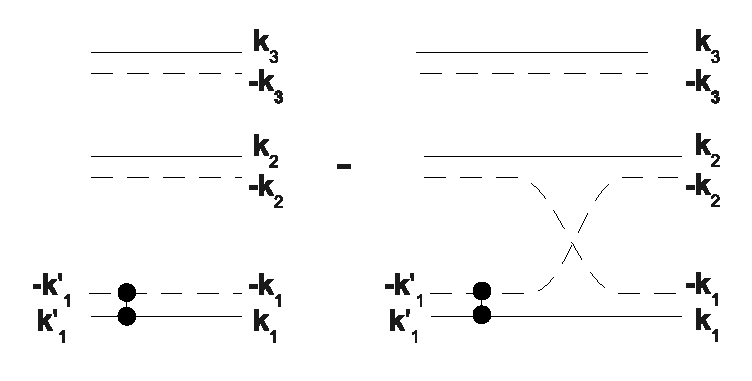
\includegraphics[width=0.4\textwidth]{threePair.eps}
Part resulting from the BCS potential acting on three pairs, as given in
Eqs. (\ref{eq:vThree},\ref{eq:vThree2}). $\left|v_{\mathbf{k} _1\mathbf{k} _2%
\mathbf{k} _3}\right> $ also contains two similar contributions as the one
visualized in this figure, obtained by circular permutation.
\end{figure}

If we come back to Eq.\eqref{eq:SchThree2}, substract $\mathbf{E}
_3\beta^{\dagger}_{\mathbf{k} _1}\beta^{\dagger}_{\mathbf{k}
_2}\beta^{\dagger}_{\mathbf{k} _3}\left|F_0\right>  $ to both sides, with $%
\mathbf{E} _3$ written as $R_1+R_2+R_3$, and multiply the resulting equation
by $w_{\mathbf{k} _1}w_{\mathbf{k} _2}w_{\mathbf{k} _3}/\left(2\epsilon_{%
\mathbf{k} _1}-R_1\right) \left(2\epsilon_{\mathbf{k} _2}-R_2\right)
\left(2\epsilon_{\mathbf{k} _3}-R_3\right) $, we find

\begin{multline}  \label{eq:SchThree3}
(H-\mathbf{E} _3)B^{\dagger}_{\mathbf{k} _1}(R_1)B^{\dagger}_{\mathbf{k}
_2}(R_2)B^{\dagger}_{\mathbf{k} _3}(R_3)\left|F_0\right>  = \\
\left\{B^{\dagger}_{\mathbf{k} _1}(R_1)B^{\dagger}_{\mathbf{k}
_2}(R_2)\left(w_{\mathbf{k} _3}\beta^{\dagger}_{\mathbf{k} _3}-\frac{Vw_{%
\mathbf{k} _3}}{2\epsilon_{\mathbf{k} _2}-R_3}\beta^{\dagger}\right) +\text{%
2 perm}\right\}  \\
\left|F_0\right>   \\
+2V\left\{B^{\dagger}_{\mathbf{k} _3}(R_3)\frac{\delta_{\mathbf{k} _1\mathbf{%
k} _2}w_{\mathbf{k} _1}}{\left(2\epsilon_{\mathbf{k} _1}-R_1\right)
\left(2\epsilon_{\mathbf{k} _1}-R_2\right) }\beta^{\dagger}_{\mathbf{k} _1}+%
\text{2 perm}\right\}  \\
\beta^{\dagger}\left|F_0\right>  
\end{multline}
To proceed, we rewrite $\left(2\epsilon_{\mathbf{k} _1}-R_1\right)
^{-1}\left(2\epsilon_{\mathbf{k} _2}-R_2\right) ^{-1}$ as $\left[%
\left(2\epsilon_{\mathbf{k} _1}-R_1\right) ^{-1}-\left(2\epsilon_{\mathbf{k}
_2}-R_2\right) ^{-1}\right] /\left(R_1-R_2\right) $ provided that $R_1\neq{}%
R_2$ and do the same for the two other products. By taking the sum over $%
\left(\mathbf{k} _1,\mathbf{k} _2,\mathbf{k} _3\right) $, we end with

\begin{multline}  \label{eq:SchThree4}
(H-\mathbf{E} _3)B^{\dagger}(R_1)B^{\dagger}(R_2)B^{\dagger}(R_3)\left|F_0%
\right>  = \\
\{B^{\dagger}(R_2)B^{\dagger}(R_3) \\
\left(1-V\sum\frac{w_{\mathbf{k} _1}}{2\epsilon_{\mathbf{k} _1}-R_1}-\frac{2V%
}{R_1-R_2}+\frac{2V}{R_3-R_1}\right)  \\
+\text{2 perm}\}\beta^{\dagger}\left|F_0\right>  
\end{multline}

This leads us to again conclude that the three-pair state $%
B^{\dagger}(R_1)B^{\dagger}(R_2)B^{\dagger}(R_3)\left|F_0\right>  $ is
eigenstate of the hamiltonian with the energy $\mathbf{E} _3=R_1+R_2+R_3$,
provided that $\left(R_1,R_2, R_3\right) $ fulfill the three equations, 
\begin{equation}
\begin{split}
1&=V\sum\frac{w_{\mathbf{k} }}{2\epsilon_{\mathbf{k} }-R_1}+\frac{2V}{R_1-R_2%
}+\frac{2V}{R_1-R_3} \\
1&=V\sum\frac{w_{\mathbf{k} }}{2\epsilon_{\mathbf{k} }-R_2}+\frac{2V}{R_2-R_3%
}+\frac{2V}{R_2-R_1} \\
1&=V\sum\frac{w_{\mathbf{k} }}{2\epsilon_{\mathbf{k} }-R_3}+\frac{2V}{R_3-R_1%
}+\frac{2V}{R_3-R_2}
\end{split}%
\end{equation}

\subsection{N pairs}

The above commutation technique can be easily extended to N pairs. As nicely
visualized by the diagrams of Figs. \ref{fig:twoP} and \ref{fig:threeP}, the
effect of the BCS potential on these N pairs splits into two sets of terms:
In one set, one pair is affected by the (1x1) scattering while the other $N-1
$ pairs stay unchanged. In the other, this pair in addition has a fermion
exchange before the interaction, with another pair, the remaining $N-2$
pairs staying unchanged. This readily shows that an increase of the number
of pairs above two, does not really change the structure of the equations
since $N-2$ pairs stay unchanged, the pair exchanging its fermions with the
pair suffering the interaction being just one among $(N-1)$ pairs.

Although the equations become more and more cumbersome to be explicitly
written, the procedure is rather straightforward once we have understood
that either $(N-1)$ or $(N-2)$ pairs stay unaffected in the process. The
general form of the N-pair eigenstate ultimately appears as 
\begin{equation}  \label{eq:SchThreeN}
(H-\mathbf{E} _N)B^{\dagger}(R_1)\cdots{}B^{\dagger}(R_N)\left|F_0\right>  =0
\end{equation}
with $\mathbf{E} _3=R_1+\cdots+R_N$, these $R_N$'s being solutions of $N$
equations like 
\begin{equation}
1=V\sum\frac{w_{\mathbf{k} }}{2\epsilon_{\mathbf{k} }-R_i}+\sum_{i\neq{j}}%
\frac{2V}{R_i-R_j}\quad\qquad \text{for}\; i=\left(1,...,N\right) 
\end{equation}

\subsection{Physical understanding}

This new derivation of the Richardson equation has the main advantage to
possibly trace back the parts in these equations which are directly linked
to the Pauli exclusion principle between fermion pairs.

From a mathematical point of view, the link is rather obvious: In the
absence of terms in $V/(R_i-R_j)$, the $N$ equations for $R_i$ reduced to
the same equation \eqref{eq:SchOne}, so that the result would be $R^0_i=%
\mathbf{E} _1$ for all $i$. The fact that the energy of $N$ pairs differs
from $N$ times the single pair energy thus comes from those $(R_i-R_j)$
differences.

Physically, the fact that $\mathbf{E} _N$ differs from $N\mathbf{E} _1$
comes from interactions between pairs. Due to the (1x1) form of the BCS
potential, interaction between pairs can only be mediated by fermion
exchanges as clear from Fig. \ref{fig:chi}. Interaction between pairs thus
is solely the result of the Pauli exclusion principle between pairs. This
Pauli blocking mathematically appears through the various $\delta_{\mathbf{p}
^{\prime}\mathbf{p} }$ factors appearing in Pauli scatterings $\lambda\left(%
\begin{smallmatrix}\vp'_2&\vp_2\\\vp_1'&\vp_1\end{smallmatrix}\right)  $. It
is then easy to mathematically trace back the $(R_i-R_j)$ differences
appearing in the Richardson equations to these $\delta$ factors.

In short, the Kronecker symbols in the Pauli scatterings of fermion pairs
result from the Pauli exclusion principle. They induce terms in $V/(R_i-R_j)$
in the Richardson equations which make the energy of $N$ pairs different
from the one of a collection of $N$ independent single pairs.

Another very interesting feature of the energy $\mathbf{E} _N$ of $N$ pairs,
this new derivation explains in a rather clear way, is the fact that the
part of the $N$ pairs energy coming from interaction, namely $\mathbf{E} _N-N%
\mathbf{E} _1$ depends on $N$ as $N(N-1)$ only. Indeed, diagram \ref%
{fig:threeP} evidences that the contribution of the (1x1) BCS potential
mixed with fermion exchanges between pairs having one degree of freedom
only, ends by producing effective scatterings which are (2x2) only. Since,
in order to have terms in $N(N-1)(N-2)$, we need topologically connected
interaction processes between 3 objects, $N(N-1)(N-2)$ terms as well as all
the higher order terms, cannot exist in the energy of $N$ Cooper pairs.

This actually is what we have found by solving these equations analytically
in the dilute limit on the single Cooper pair scale. In this limit, the
energy of N pairs was shown to read as 
\begin{equation}  \label{eq:en}
\mathbf{E} _N=N\mathbf{E} _1+N(N-1)\left(\frac{1}{\rho_0} +\frac{\epsilon_c}{%
N_\Omega}\right) 
\end{equation}
$\rho_0$ is the density of pair states in the potential layer, $%
N_\Omega=\rho_0\Omega$ is number of states in the layer, and $\epsilon_c$ is
the single pair binding energy. By writing it as $\epsilon_c=N_\Omega%
\epsilon_V$, this energy also reads, for $\mathbf{E} _1=2\epsilon_{F_0}-%
\epsilon_c$ where $\epsilon_{F_0}$ is the Fermi level of the frozen sea $%
\left|F_0\right> $ 
\begin{equation}
\mathbf{E} _N=2N\left[\epsilon_{F_0}+\frac{N(N-1)}{\rho_0}\right]
-N\epsilon_V\left(N_V-\frac{N-1}{N_\Omega}\right) 
\end{equation}
The first term corresponds to the kinetic energy of $N$ pairs added to $%
\epsilon_{F_0}$, i.e., 
\begin{equation}
2\epsilon_{F_0}+\left(2\epsilon_{F_0}+1/\rho_0\right)
+\cdots\;+\left(2\epsilon_{F_0}+(N-1)/\rho_0\right) 
\end{equation}
The second term evidences the fact that the Cooper pair binding energy
linearly decreases with pair number, this energy being proportional to the
number of empty states $N_V-(N-1)$ filling the potential.

This brings the binding energy down to $\epsilon_c/2$ in the BCS
configuration, i.e., when pairs fill half the potential layer. Actually, the
result fully agrees with the BCS condensation energy, ??? to read 
\begin{equation}
E_{\text{super}}-E_\text{normal}=\frac{1}{2} \rho_0\Delta^2=\frac{%
\rho_0\Omega}{2}\frac{2\Omega{e^{-2/\rho_0V}}}{2}
\end{equation}
In spite of the fact that Eq. \eqref{eq:en} has up to now been derived
within the dilute limit only, it turns out that it is valid over the whole
density range. This validity is a bare result of the existence of $(2\times2)
$ effective scatterings only between fermion pairs, this argument having
nothing to do with the pair density large or small on the single Cooper pair
scale.

\section{Richardson exact eigenstate versus BCS ansatz \label{sec:conn}}

Another very interesting result the Richardson procedure generates is the 
\emph{exact} form of the eigenstate, namely 
\begin{equation}
B^{\dagger}(R_1)\cdots{}B^{\dagger}(R_N)\left|F_0\right>  
\end{equation}
with $B^{\dagger}(R)$ given by Eq. \eqref{eq:B}. The fact that by
construction all the $R_i$'s are different, strongly questions the standard
BCS ansatz. For Cooper pair wave function $\left(B^{\dagger}\right)
^N\left|F_0\right>  $ with \emph{all} the pairs condensed into the same
state.

To discuss this problem on precise grounds, let us start with two pairs. In
a previous work\cite{combescotBCS}, we have shown, that the two "Richardson
energies" then read $R_1=R+iR^{\prime}$ and $R_2=R-i{}R^{\prime}$ with $R$
and $R^{\prime}$ real, their precise values being $R\approx\epsilon_c+1/%
\rho_0+\epsilon_c/N\Omega$ and $R^{\prime}=\sqrt{2\epsilon_c/\rho_0}$ in the
large sample limit, i.e. for $1/\rho_0$ small. By noting that 
\begin{multline}
B^{\dagger}(R_1)B^{\dagger}(R_2)= \\
\left[B^{\dagger}(R)+B^{\dagger}(R_1)-B^{\dagger}(R)\right] \left[%
B^{\dagger}(R)+B^{\dagger}(R_2)-B^{\dagger}(R)\right] 
\end{multline}
we get from eq \eqref{eq:B} 
\begin{equation}
B^{\dagger}(R_1)B^{\dagger}(R_2)=\left[B^{\dagger}(R)\right]
^2+{R^{\prime}}^2\left\{C^{\dagger}_+C^{\dagger}_--2B^{\dagger}(R)D^{\dagger}%
\right\} 
\end{equation}
where we have set 
\begin{align}
C^{\dagger}_{\pm}&=\sum\frac{w_\vk}{\left(2\epsilon_\vk-R\right)
\left(2\epsilon_\vk-R\pm{}iR^{\prime}\right) }\beta^{\dagger}_\vk \\
D^{\dagger}&=\sum\frac{w_\vk}{\left(2\epsilon_\vk-R\right) \left[%
\left(2\epsilon_\vk-R\right) ^2+{}{R^{\prime}}^2\right] }\beta^{\dagger}_\vk
\end{align}
So that at first order in sample volume, i.e., in $1/\rho_0$, we find since $%
N_\Omega=\rho_0\Omega$ 
\begin{multline}  \label{eq:BB}
B^{\dagger}(R_1)B^{\dagger}(R_2)-\left[B^{\dagger}(\frac{\mathbf{E} _2}{2})%
\right] ^2\approx \frac{2\epsilon_c}{\rho_0} \\
\left\{-2B^{\dagger}(\mathbf{E} _1)\sum\frac{w_\vk}{\left(2\epsilon_\vk-%
\mathbf{E} _1\right) ^3}\beta^{\dagger}_\vk +\left[\sum\frac{w_\vk}{%
\left(2\epsilon_\vk-\mathbf{E} _1\right) ^2}\beta^{\dagger}_\vk\right]
^2\right\}  \\
+O(\frac{1}{\rho_0^2} )
\end{multline}
The above result shows that $B^{\dagger}(R_1)B^{\dagger}(R_2)$ can be
written as $\left(B^{\dagger}(\mathbf{E} _2/2)\right) ^2$ provided that we
drop all $1/\rho_0$ terms. However $B^{\dagger}$ then reduces to $%
B^{\dagger}(\mathbf{E} _1)$. This barely corresponds to consider the
two-pair eigenstate as the product of two non-interacting single pairs. If
instead, we want, in the condensed pair creation operator, include the
change from one to two pairs induced by Pauli blocking which brings the
energy per pair from $\mathbf{E} _1$ to $\mathbf{E} _2/2=\mathbf{E}
_1+1/\rho_0+\epsilon_c/N_\Omega$, we are led to replace $B^{\dagger}(R_1)B^{%
\dagger}(R_2)$ by $\left(B^{\dagger}(\mathbf{E} _2/2)\right) ^2$. This
however is inconsistent because we then keep in this condensed pair
operator, contribution in $1/\rho_0$ which are as large as the ones we drop
in the LHS of eq \eqref{eq:BB}. In the case of two pairs, the replacement of
the exact eigenstate $B^{\dagger}(R_1)B^{\dagger}(R_2)\left|F_0\right>  $ by
a BCS-like condense state $\left(B^{\dagger}(\mathbf{E} _2/2)\right)
^2\left|F_0\right>  $ th  us is inconsistent.

It is actually claimed that the BCS ansatz is valid in the thermodynamical
limit, i.e., for $N$ and $V$ both very large. Derivation of the "validity"
is in fact with restrict to the energy only. We fully agree that the BCS
ansatz give the correct energy since the energy obtained using this ansatz
is just the one we have derived from the exact Richardson procedure. However
agreement on the energy by no mean proves agreement on the wave function.
Many examples have been given in the past with wave function very different
from the exact one, while giving the correct energy.

The possible replacement of $B^{\dagger}(R_1)\cdots{}B^{\dagger}(R_N)%
\left|F_0\right>  $ by $\left(B^{\dagger}\right) ^N\left|F_0\right>  $ is
actually crucial to support the overall picture we all have of
superconductivity, with all the pairs in the same state, as an army of
little solders, all walking similarly.

\section{Conclusion}

We have rederived the Richardson equations using a commutation technique for
free electron pairs with zero total momentum similar to the one we have
developed for composite boson excitons. Almost half a century ago,
Richardson has succeeded to write the \emph{exact} eigenstate for an
arbitrary number $N$ of pairs in a compact form in terms of $N$ energy-like
quantities $R_1,..., R_N$, which are solution of $N$ coupled non-linear
equations. This $2N$ many-body problem is exactly solvable provided that the
interaction potential is taken as a BCS-like potential having a separable
scattering $v_{\mathbf{k} ^{\prime}\mathbf{k} }=-V\,w_{\mathbf{k}
^{\prime}}w_{\mathbf{k} }$ with $w_{\mathbf{k} }$ moreover such that $%
w_\vk^2=1$. Note that these assumptions are already those necessary to get
the energy of a single pair in the compact form obtained by Cooper.
Richardson managed to extend Cooper exact solution to $N$ pairs by
decoupling them through rewriting their energy $E_N$ as $R_1+\cdots+R_N$.

The new composite boson derivation we here propose, allows us to trace back
the physical origin of the various terms of these equations. It in
particular clearly shows that $N$ pairs differ from $N$ independent single
pairs, due to Pauli exclusion principle only. This Pauli blocking also
enforces the $R_i$ energy-like parameters to be different, namely the exact $%
N$-pair eigenstate different from the BCS ansatz. ?????? the diagrammatic
representation of this derivation evidences that, due to the fact that pairs
with zero total momentum, do have one degree of freedom only, they only have 
$2\times2$ scatterings within the $1\times1$ BCS potential. This explains
why the $N$ pair energy has terms in $N$ and $N(N-1)$ but not in $N(N-1)(N-2)
$ and so on.

One of us (M.C.) wishes to thank the University of Illinois at
Urbana-Champaign, and Tony Leggett in particular, for a month invitation at
the Institute for Condensed Matter Physics where most of this work has been
done.

\begin{thebibliography}{Combescot et~al.(2008)Combescot, Betbeder-Matibet,
and Dubin}
\bibitem{} \expandafter\ifx\csname natexlab\endcsname\relax

\fi
\expandafter\ifx\csname bibnamefont\endcsname\relax

\fi
\expandafter\ifx\csname bibfnamefont\endcsname\relax

\fi
\expandafter\ifx\csname citenamefont\endcsname\relax

\fi
\expandafter\ifx\csname url\endcsname\relax

\fi
\expandafter\ifx\csname urlprefix\endcsname\relax

\fi
\providecommand{\bibinfo}[2]{#2} \providecommand{\eprint}[2][]{\url{#2}}

\bibitem[Bardeen et~al.(1957)Bardeen, Cooper, and Schrieffer]{BCS} %
\bibinfo{author}{\bibfnamefont{J.}~\bibnamefont{Bardeen}},  %
\bibinfo{author}{\bibfnamefont{L.~N.} \bibnamefont{Cooper}},  and 
\bibinfo{author}{\bibfnamefont{J.~R.}
  \bibnamefont{Schrieffer}}, \bibinfo{journal}{Physical Review}  \textbf{%
\bibinfo{volume}{106}}, \bibinfo{pages}{162} (\bibinfo{year}{1957}).

\bibitem[Richardson(1963)]{Richardson1} \bibinfo{author}{%
\bibfnamefont{R.~W.} \bibnamefont{Richardson}},  \bibinfo{journal}{physics
letters} \textbf{\bibinfo{volume}{3}},  \bibinfo{pages}{277} (%
\bibinfo{year}{1963}).

\bibitem[Richardson and Sherman(1964)]{Richardson2} \bibinfo{author}{%
\bibfnamefont{R.~W.} \bibnamefont{Richardson}}  and \bibinfo{author}{%
\bibfnamefont{N.}~\bibnamefont{Sherman}},  \bibinfo{journal}{Nucl. Phys.} 
\textbf{\bibinfo{volume}{52}},  \bibinfo{pages}{221} (\bibinfo{year}{1964}).

\bibitem[Combescot et~al.(2008)Combescot, Betbeder-Matibet, and Dubin]%
{CobosonPhysicsReports} \bibinfo{author}{\bibfnamefont{M.}~%
\bibnamefont{Combescot}},  \bibinfo{author}{\bibfnamefont{O.}~%
\bibnamefont{Betbeder-Matibet}},  and \bibinfo{author}{\bibfnamefont{F.}~%
\bibnamefont{Dubin}},  \bibinfo{journal}{Physics Reports} \textbf{%
\bibinfo{volume}{463}},  \bibinfo{pages}{215} (\bibinfo{year}{2008}).

\bibitem[Combescot and Betbeder-Matibet(2007)]{CobosonCalculation} %
\bibinfo{author}{\bibfnamefont{M.}~\bibnamefont{Combescot}} and  %
\bibinfo{author}{\bibfnamefont{O.}~\bibnamefont{Betbeder-Matibet}},  %
\bibinfo{journal}{The European Physical Journal B}  \textbf{%
\bibinfo{volume}{55}}, \bibinfo{pages}{63} (\bibinfo{year}{2007}).

\bibitem[Pogosov1 et~al.()Pogosov1, Combescot, and Crouzeix]{combescotBCS} %
\bibinfo{author}{\bibfnamefont{W.~V.} \bibnamefont{Pogosov1}}, %
\bibinfo{author}{\bibfnamefont{M.}~\bibnamefont{Combescot}}, and %
\bibinfo{author}{\bibfnamefont{M.}~\bibnamefont{Crouzeix}}.
\end{thebibliography}

\end{document}
